	\documentclass[10pt,oneside]{CBFT_book}
	% Algunos paquetes
	\usepackage{amssymb}
	\usepackage{amsmath}
	\usepackage{graphicx}
	\usepackage{bm}
% 	\usepackage{libertine}
	\usepackage[bold-style=TeX]{unicode-math}
	\usepackage{lipsum}

	\usepackage{natbib}
	\setcitestyle{square}

	\usepackage{polyglossia}
	\setdefaultlanguage{spanish}


	\usepackage{CBFT.estilo} % Cargo la hoja de estilo

	% Tipografías
	% \setromanfont[Mapping=tex-text]{Linux Libertine O}
	% \setsansfont[Mapping=tex-text]{DejaVu Sans}
	% \setmonofont[Mapping=tex-text]{DejaVu Sans Mono}

	%===================================================================
	%	DOCUMENTO PROPIAMENTE DICHO
	%===================================================================

\begin{document}

% =================================================================================================
\chapter{Teorema de Green}
% =================================================================================================

% =================================================================================================
\section{Imágenes y método de Green}
% =================================================================================================

El método de las imágenes es un procedimiento gráfico de encontrar problemas equivalentes simulando
con cargas extras (cargas imagen) las condiciones de contorno.

\begin{figure}[htb]
	\begin{center}
	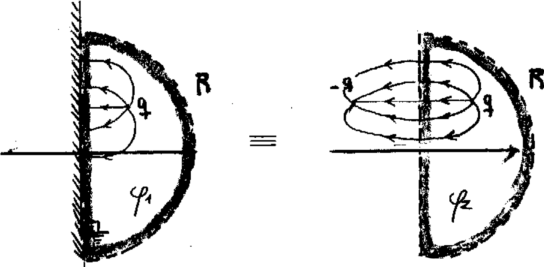
\includegraphics[width=0.6\textwidth]{images/fig_ft1_imagegreen1.pdf}	 
	\end{center}
	\caption{}
\end{figure} 

Los problemas que ilustra la figura satisfacen iguales condiciones de contorno en el recinto punteado,
entonces sus soluciones internas son la misma: $\phi_1 = \phi_2$ por unicidad.

\subsection{El Método de Green}

El concepto tras el método de Green es evaluar el $\phi$ de una carga puntual ante cierta configuración
de contornos conductores. Es una excitación elemental.

Restando entre sí
\[
	\Nabla\cdot(\phi\Nabla\psi) = \phi\lapm{\psi} + \Nabla\phi\cdot\Nabla\psi
\]
y
\[
	\Nabla\cdot(\psi\Nabla\phi) = \psi\lapm{\phi} + \Nabla\psi\cdot\Nabla\phi
\]
e integrando ambos miembros y utilizando el teorema de la divergencia, se llega a
\[
	\int_V \left[ \phi\lapm{\psi} - \psi\lapm{\phi}\right] dV =
	\int_S \left[ \phi\Nabla\psi - \psi\Nabla\phi \right] dS,
\]
que es la segunda identidad de Green.

Consideremos lo que llamaremos caso A, según vemos en figura, caracterizado según
\[
	\rho_{int} \qquad \vb{x}'\in R, \vb{x}\in R
\]
\begin{figure}[htb]
	\begin{center}
	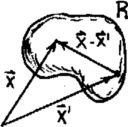
\includegraphics[width=0.2\textwidth]{images/fig_ft1_imagegreen2.pdf}	 
	\end{center}
	\caption{}
\end{figure} 
\[
	\psi = \frac{1}{|\vb{x}-\vb{x}'|} \qquad \lapm{\psi} = -4\pi \delta(\vb{x}-\vb{x}')
\]
\[
	-\phi(\vb{x})4\pi + \int_V 4\pi \frac{\rho(\vb{x}')}{|\vb{x}-\vb{x}'|} \; dV' =
	\int_S \left( \phi\dpar{\psi}{n}-\frac{1}{|\vb{x}-\vb{x}'|}\dpar{\phi}{n}\right)\; dS 
\]
donde estamos usando la abreviatura $\Nabla\phi\cdot\vb{n}=\partial\phi/\partial n$ que es la
derivada normal en la superficie. Despejando
\[
	\phi(\vb{x}) = \int_V \frac{\rho(\vb{x}')}{|\vb{x}-\vb{x}'|} \; dV' +
	\frac{1}{4\pi} \int_S \left( \frac{1}{|\vb{x}-\vb{x}'|}\dpar{\phi}{n} -\phi\frac{\partial}{\partial 
n} \left[\frac{1}{|\vb{x}-\vb{x}'|} \right] \right)\; dS ,
\]
donde la primer integral es debido a las cargas internas y la segunda al efecto de las cargas
fuera del reciento $R$.

Recordemos que las condiciones tipo Dirichlet corresponden a $\phi|_S$ y las tipo Neumann a
$\partial\phi/\partial \hat{n}|_S$.

El caso B, según figura, corresponde a
\[
	\rho_{int} \qquad \vb{x}'\notin R, \vb{x}\in R
\]
y 
\[
	\int_V \frac{\rho(\vb{x}')}{|\vb{x}-\vb{x}'|} \; dV' = 
	\frac{1}{4\pi} \int_S \left( \phi\frac{\partial}{\partial n} \left[\frac{1}{|\vb{x}-\vb{x}'|} \right]
	- \frac{1}{|\vb{x}-\vb{x}'|}\dpar{\phi}{n}  \right)\; dS ,
\]
la integral de superficie proviene de las cargas fuera de $R$ que producen campo en el interior
$R$.

\begin{figure}[htb]
	\begin{center}
	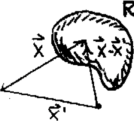
\includegraphics[width=0.2\textwidth]{images/fig_ft1_imagegreen3.pdf}	 
	\end{center}
	\caption{}
\end{figure} 

Hemos tomado $\psi=1/|\vb{x}-\vb{x}'|$ que verifica [1]; interpretándose $\psi$ como el potencial
de una carga puntual unitaria.

\[
	\lapm{\frac{1}{|\vb{x}-\vb{x}'|}} = - 4\pi \delta( |\vb{x}-\vb{x}'| )
\]
podemos tomar
\[
	G \equiv \frac{1}{|\vb{x}-\vb{x}'|} + f( \vb{x}, \vb{x}')
\]
donde $G$ es la función de Green.

\[
	\lapm{G} = -4\pi  \delta( \vb{x}, \vb{x}' ) + \lapm{f}
\]
donde $F$ satisface Laplace (si el reciento no incluye a $\vb{x}'$).
Con $\lapm{f( \vb{x}, \vb{x}' )}$.

Entonces $f( \vb{x}, \vb{x}' )$ representan la o las imágenes necesarias para que
$G$ cumpla el contorno necesario $G_D|_S=0$.


% =================================================================================================
\section{Funciones de Green}
% =================================================================================================

\be
	\phi(\vb{x}) = \int_{V'} G(\vb{x},\vb{x}') \rho(\vb{x}')  \; dV' +
	\frac{1}{4\pi} \int_{S'} \left( G(\vb{x},\vb{x}')\dpar{\phi}{n} -\phi\frac{\partial}{\partial 
	n} G(\vb{x},\vb{x}') \right)\; dS' ,
	\label{green1}
\ee
Pero para poder utilizar \eqref{green1} necesito tener un solo tipo de condiciones de contorno,
de manera que según sean
\[
	\textrm{Dirichlet} \quad 	\begin{cases}
				G_D : \lapm{G_D} = -4\pi \delta(\vb{x},\vb{x}') \\
				G_D |_{contorno de R} = 0  \\
				\phi|_S \\
				\phi(\vb{x}) = \displaystyle \int_{V'} G_D \rho \; dV' - \frac{1}{4\pi}
				\int_{S} \phi|_S\frac{\partial}{\partial n} G_D \; dS'
			\end{cases}
\]
donde la condición de contorno de $G$ equivale, en el contexto físico del electromagnetismo, a
reemplazar el contorno por un conductor metálico puesto a tierra.
Entonces $G$ es el potencial de la configuración de conductores con el contorno puesto a tierra
frente a una carga puntual con magnitud unitaria.

La función de Green da la geometría del problema.

\[
	\dpar{\phi_1}{n}|_S - \dpar{\phi_2}{n}|_S = -4\pi\sigma \qquad \qquad \phi_2|_S = \phi_1|_S
\]

\[
	\textrm{Neumann} \quad 	\begin{cases}
				G_N : \lapm{G_N} = -4\pi \delta(\vb{x},\vb{x}') \\
				\Nabla G_N \cdot \hat{n}|_S = -\frac{4\pi}{S}  \\
				\left.\dpar{\phi}{n}\right|_S \\
				\phi(\vb{x}) = \displaystyle <\phi>|_S + \int_{V'} G_N \rho \; dV' + 
				\frac{1}{4\pi} \int_{S} G_N|_S \dpar{G_N}{n} \; dS
			\end{cases}
\]

\subsection{Green para el problema externo de una esfera}

En este problema las condiciones adecuadas son las de Dirichlet, ver Figura
\begin{figure}[htb]
	\begin{center}
	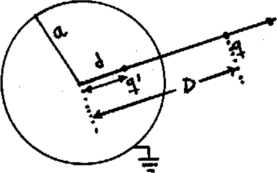
\includegraphics[width=0.4\textwidth]{images/fig_ft1_green1.pdf}	 
	\end{center}
	\caption{}
\end{figure} 
y podemos escribir la función de Green como 
\[
	G = \frac{1}{|\vb{r} - D\hat{r}'|} - \frac{a/D}{|\vb{r} - a^2/D\hat{r}'|} \qquad G|_{r=a}
\]
sujeta a que 
\[
	q' = -q a/D \qquad d = a^2/D
\]
\begin{figure}[htb]
	\begin{center}
	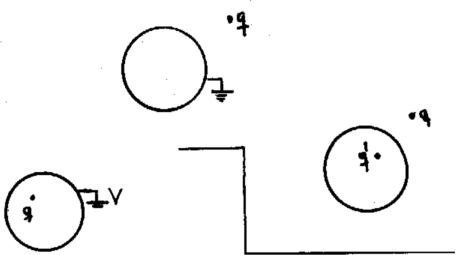
\includegraphics[width=0.6\textwidth]{images/fig_ft1_green2.pdf}	 
	\end{center}
	\caption{$G_D$ es el potencial de la configuración (a) y se evalúa teniendo en cuenta la
	otra (b) que se resuelve casualmente por imágenes. La (c) se resuelve alterando las condiciones.}
\end{figure} 

El caso (c) de la Figura se resuelve con 
\[
	-\frac{V}{4\pi} \int_S \dpar{G}{n} dS = -\frac{V}{4\pi} \int_S \Nabla G\cdot d\vb{S} =
	-\frac{V}{4\pi} \int_V \lapm{G} \: dV	
\]
\[
	= -\frac{V}{4\pi} (-4\pi)\int_V \delta(\vb{x}-\vb{x}') \: dV	= V 
\]

\section{Algunos campos}

En distribuciones infinitas de carga la integral de Poisson diverge pero ello se debe a que en
realidad no existen distribuciones infinitas de carga.
\begin{figure}[thb]
	\begin{center}
	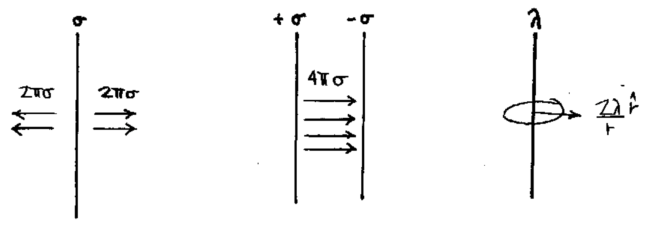
\includegraphics[width=0.8\textwidth]{images/fig_ft1_campohilos.pdf}	 
	\end{center}
	\caption{}
\end{figure} 

\section{Notas método de Green}

Función de Green libre (sin contornos) lleva directo a la integral de Poisson
\[
	G(\vb{x}, \vb{x}') = \frac{1}{|\vb{x} - \vb{x}'|}
\]
entonces 
\[
	\phi(\vb{x}) = \int_V \rho \:G \:dV = \int_{V'} \frac{ \rho(\vb{x}) }{|\vb{x}-\vb{x}'|} dV'
\]
\[
	\nabla^2 \left( \frac{1}{|\vb{x} - \vb{x}'|} \right) = 4\pi \delta(\vb{x}-\vb{x}')
\]
\[
	G(\vb{x}, \vb{x}') =  \frac{1}{|\vb{x} - \vb{x}'|} + f(\vb{x}, \vb{x}') \qquad 
	\textrm{con} \quad \lapm{f}(\vb{x}, \vb{x}') = 0 \quad \textrm{si} \quad \vb{x}\neq\vb{x}'
\]

Para condiciones de Neumann se toma:
\[
	\Nabla G_N|_S = -\frac{4\pi}{S} = \left. \dpar{G}{n} \right|_S
\]
la integral 
\[
	- \frac{1}{4\pi} \int_S \phi|_S \left.\dpar{G}{n}\right|_S  dS
\]
no se puede anular con 
\[
	\left.\dpar{G}{n}\right|_S = 0
\]
salvo que el volumen de integración no contenga a $\vb{x}=\vb{x}'$ en cuyo caso:
se excluye $\vb{x}=\vb{x}'$ de la integración.
\[
	- \frac{1}{4\pi} \int_S \phi|_S \left.\dpar{G}{n}\right|_S  dS =
	\frac{1}{S} \int_S \phi|_S dS = <\phi>|_S
\]
que es el valor promedio de $\phi$ en la superficie $S$.

Se suele tomar la superficie $S \to \infty$ de modo que resulte nulo $<\phi>|_S$.
Se toma el volumen $V$ rodeado por dos superficies una cerrada y finita y la otra
en infinito entonces
\[
	<\phi>|_S = 0 \qquad \qquad \left. \dpar{G}{n}\right|_S = 0
\]
esto es el llamado {\it problema exterior}.

% =================================================================================================
\section{Condiciones de contorno}
% =================================================================================================

La ley de Gauss nos dice
\[
	\int \vb{E} \cdot d\vb{S} = 4 \pi Q_n
\]
para el cilindrito de la figura
\[
	( \vb{E}_2 - \vb{E}_1 )\cdot \hat{n} \Delta S = 4 \pi \sigma \Delta S 
\]
\[
	( \vb{E}_2 - \vb{E}_1 )\cdot \hat{n} = 4 \pi \sigma 
\]
\[
	\rotorm{E} = 0 \Rightarrow \int_\Gamma \vb{E} \cdot d\vb{\ell} = 0 =
	( \vb{E}_2 - \vb{E}_1 )\cdot d\vb{\ell}  = ( \vb{E}_1 + \vb{E}_2 ) \cdot \hat{n}\times\hat{\eta} d\ell
\]
donde esto vale en electrostática (nula la integral de línea del campo \vb{E}) y además
\[
	\hat{n}\times\hat{\eta} = \frac{d\vb{\ell}}{d\ell} 
\]

\begin{figure}[htb]
	\begin{center}
	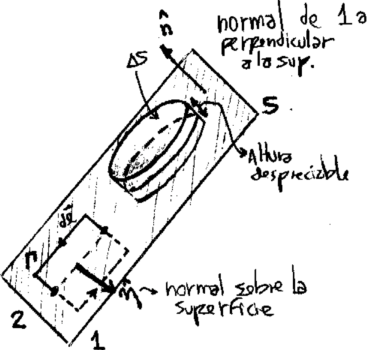
\includegraphics[width=0.4\textwidth]{images/fig_ft1_contorno1.pdf}	 
	\end{center}
	\caption{}
\end{figure} 
y puesto que vale la permutación
\[
	0 = ( -\vb{E}_2 + \vb{E}_1 )\cdot(\hat{n}\times\hat{\eta}) \longrightarrow 
	0 = \hat{\eta} \cdot ( ( -\vb{E}_2 + \vb{E}_1 ) \times \hat{n} )
\]

de modo que la componente tangencial es continua y entonces
\[
	\hat{n} \times ( \vb{E}_2 - \vb{E}_1 ) = 0
\]
\[
	E_{2\hat{n}} - E_{1\hat{n}} = 4 \pi \sigma \qquad \qquad E_{2\hat{t}} -E_{1\hat{t}} = 0
\]
\[
	-\Nabla\phi_2\cdot\hat{n} + \Nabla\phi_1\cdot\hat{n} = 4 \pi \sigma
\]
\[
	\frac{\Nabla(\phi_2-\phi_1)\cdot \hat{n}}{4 \pi} = \sigma
\]
\[
	\sigma = \frac{1}{4\pi}\dpar{(\phi_1-\phi_2)}{n}
\]
esta es la densidad de carga inducida sobre la frontera entre medios.

Para los medios magnéticos
\[
	\rotorm{H} = \frac{4 \pi}{c} \vb{J}_l
\]
\[
	\int_S (\rotorm{H}) \cdot d\vb{S} = \int_S \frac{4 \pi}{c} \vb{J}_l \cdot d\vb{S} = 
	\frac{4 \pi}{C} \vb{g}_l\cdot \hat{s} d\ell
\]
donde hicimos la transformación
\[
	\int \vb{H}\cdot d\ell = (\vb{H}_2-\vb{H}_1)\cdot d\ell
\]
y donde recordemos que la altura de $\Gamma$ tiene a cero.
\[
	\frac{4 \pi}{c} \vb{g}_l \cdot \vb{s} = ( -\vb{H}_2 + \vb{H}_1 )\cdot( \hat{n} \times \hat{s} ) d\ell
\]
\[
	\frac{4 \pi}{c} \vb{g}_l \cdot \vb{s} \; d\ell = (\vb{H}_1 -\vb{H}_2 \times \hat{n})\cdot \hat{s} 
d\ell
\]

\begin{figure}[htb]
	\begin{center}
	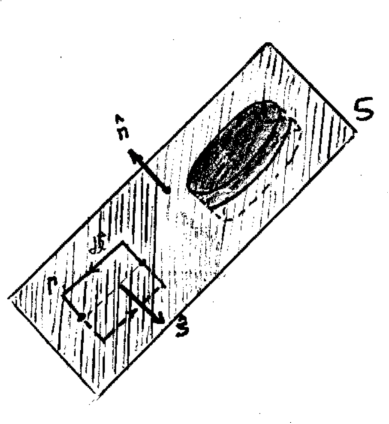
\includegraphics[width=0.4\textwidth]{images/fig_ft1_contorno2.pdf}	 
	\end{center}
	\caption{}
\end{figure} 

de manera que 
\[
	\frac{4 \pi}{c} \vb{g}_l = \hat{n} \times ( \vb{H}_2 - \vb{H}_1 )
\]
\[
	\hat{n}\times\hat{s} = \frac{d\vb{\ell}}{d\ell} 
\]
\[
	B_{2\hat{n}} - B_{1\hat{n}} = 0 \qquad \qquad H_{2\hat{t}} - H_{1\hat{t}} = \frac{4 \pi}{c} g_l
\]
\[
	\int_S \vb{B}\cdot d\vb{S} = 0 \Rightarrow (\vb{B}_2 - \vb{B}_1 )\cdot\hat{n} = 0
\]

% =================================================================================================
\section{Desarrollo multipolar}
% =================================================================================================

\[
	\phi(\vb{x}) = \int_{V'} \frac{\rho(\vb{x})}{|\vb{x}-\vb{x}'|} \; dV'
\]
Cuando la expresión es muy complicada podemos desarrollarla en una serie de potencias
\[
	\phi(\vb{x}) = \frac{Q}{|\vb{x}|} + \frac{\vb{x}\cdot\vb{p}}{|\vb{x}|^3} +
	\sum_{i,j}^3 \frac{1}{2|\vb{x}|^5} x_i Q_{ij} x_j
\]
donde está centrado en el origen de coordenadas. El último término, matricialmente sería
\[
	\frac{1}{2} \frac{\vb{x}^t Q \vb{x}}{|\vb{x}|^5}
\]
y es el término cuadrupolar.

Los momentos son el momento dipolar,
\[
	\vb{p} = \int_V \vb{x} \: \rho(\vb{x}) \: dV
\]
el momento monopolar
\[
	Q = \int_V \rho(\vb{x}) dV
\]
que es la carga total, y el momento cuadrupolar
\[
	Q_{ij} = \int_V  \rho(\vb{x}) \left[ 3 x_i x_j - \delta_{ij} |\vb{x}|^2 \right] \: dV
\]

El momento cuadrupolar refleja apartamiento de la esfera perfecta, los momentos dipolar y cuadrupolar
indican desbalance de carga.
Asimismo $Q_{ij} = Q_{ji}$ es simétrico por ser producto de vectores polares.
Es siempre diagonalizable. Tiene traza nula,
\[
	Q_{xx} + Q_{yy} + Q_{zz}  = 0
\]
se da también que $Q_{ij} (i\neq j)$ mide desbalance lejos de los ejes.
Una esfera con $\rho$ uniforme tiene todos los momentos multipolares nulos salvo el monopolo.

\begin{figure}[htb]
	\begin{center}
	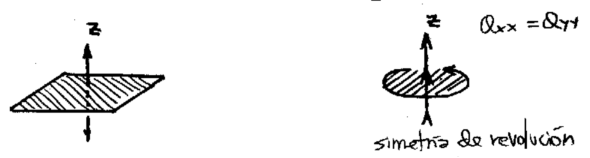
\includegraphics[width=0.8\textwidth]{images/fig_ft1_multipolo2.pdf}	 
	\end{center}
	\caption{}
\end{figure}

Una simetría de reflexión implica que el $\vb{p}_\perp = 0$ donde la notación significa perpendicular
al plano. Esto es así porque no hay desbalance. Para una simetría de revolución $Q_{xx}=Q_{yy}$ entonces
el $Q_{ij}$ puede darse con un sólo número.

Si en una distribución dada, los momentos multipolares hasta el orden $\ell -1$ son nulos entonces
el momento multipolar de orden $\ell$ no depende del origen de coordenadas.

\begin{figure}[htb]
	\begin{center}
	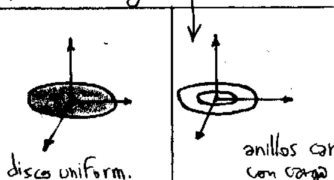
\includegraphics[width=0.6\textwidth]{images/fig_ft1_multipolo3.pdf}	 
	\end{center}
	\caption{}
\end{figure}

En la figura vemos que no ambos no tienen desbalance de carga respecto del origen; el disco uniformemente
cargado tendrá monopolo no nulo y dipolo nulo (siempre respecto del origen), los anillos cargados con carga
opuesta tendrán monopolo y dipolo nulos (respecto del origen y de cualquier otro punto). Pero si muevo las
distribuciones se tendrá desbalance el disco pero no los anillos.

\begin{figure}[htb]
	\begin{center}
	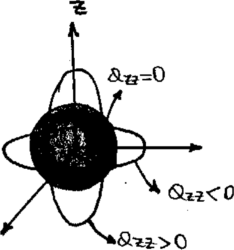
\includegraphics[width=0.3\textwidth]{images/fig_ft1_multipolo4.pdf}	 
	\end{center}
	\caption{}
\end{figure}

Para átomos en general son monopolo, dipolo neutros; el cuadrupolo se da con un solo número. 
En la Figura tenemos un elipsoide con densidad de carga $\rho$ uniforme. Tiene simetría de revolución
de modo que el momento cuadripolar es un número. $Q_{zz} = 0 $ puesto que una esfera no tiene
desbalance, entonces $\overleftrightarrow{Q} = 0 $ 


% =================================================================================================
\section{Dipolo eléctrico}
% =================================================================================================

\[
	\phi(\vb{x}) = \frac{ \vb{p}\cdot\vb{x} }{|\vb{x}|^3} 
\]
si está en el origen, y
\[
	\phi(\vb{x}) = \frac{ \vb{p}\cdot(\vb{x}-\vb{x}_0) }{|\vb{x} - \vb{x}_0|^3} 
\]
si está en un punto $\vb{x}_0$
\[
	\vb{E}(\vb{x}) = \frac{3 \vb{p}\cdot\hat{n} }{|\vb{x} - \vb{x}_0|^3}  \hat{n} - 
		\frac{ \vb{p} }{|\vb{x} - \vb{x}_0|^3}	
\]
donde debemos notar que \vb{p} no depende de \vb{x}.

\begin{figure}[htb]
	\begin{center}
	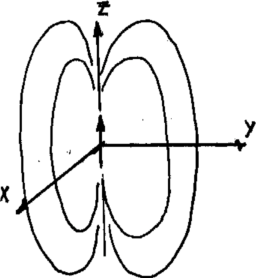
\includegraphics[width=0.3\textwidth]{images/fig_ft1_dipolar2.pdf}	 
	\end{center}
	\caption{Dipolo centrado en el origen.}
\end{figure}

\[
	\phi(\vb{x}) = \frac{p\hat{z}\cdot r\hat{r}}{r^3} = \frac{p}{r^2} \cos(\theta)
\]
siendo 
\[
	\hat{n} = \frac{\vb{x}-\vb{x}_0}{|\vb{x}-\vb{x}_0|}
\]
\[
	\vb{E}(r,\theta) = \frac{2 p\cos(\theta)}{r^3} \hat{r} + \frac{p\sin(\theta)}{r^3} \hat{\theta}
\]
tiene simetría de revolución, puesto que no depende de $\hat{\phi}$.

Las líneas de campo cuplen que $d\vb{\ell}$ a través de una línea de campo es tal que 
\[
	d\vb{\ell} \parallel \vb{E} \quad \Rightarrow \quad  \vb{E} \times d\vb{\ell}  = 0
\]
la línea de campo sigue la dirección del campo. En el caso del dipolo no tendrán componente en
$\hat{\phi}$ (como es de esperar).

\subsection{Inteacción de un campo externo con una distribución de carga}

Si tenemos un campo \vb{E} con sus fuentes lejos,

\begin{figure}[htb]
	\begin{center}
	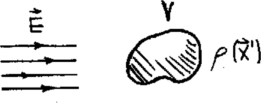
\includegraphics[width=0.4\textwidth]{images/fig_ft1_dipolar3.pdf}	 
	\end{center}
	\caption{}
\end{figure}

y que cumple $\divem{E}=0$ y $\rotorm{E}=0$ (irrotacionalidad), se da la siguiente fuerza sobre la distribución
\[
	\vb{F} = \int_V \rho(\vb{x}) \: \vb{E}(\vb{x}) \: dV,
\]
y si \vb{E} no varía demasiado en $V$, entonces podemos representar bien por una serie
\[
	E^\ell(\vb{x}) = E^\ell + x_j \partial_j E^\ell + \frac{1}{2} x_j x_k \partial_j\partial_k E^\ell
\]
entonces 
\[
	F_i = \int_V \rho E_i dV \approx E_i \int_V \rho dV + \int_V \rho  x_j \partial_j E_i dV +
		\frac{1}{2} \int_V \rho x_j x_k \partial_j\partial_k E_i dV 
\]
o bien 
\[
	F_i = \int_V \rho E_i dV \approx E_i q + (\vb{p}\cdot\Nabla) E_i  +
		\vb{x}\cdot\left[ (\vb{x}\cdot\Nabla)\Nabla E_i\right]
\]
de lo cual extraemos que el campo interactúa con la carga, el gradiente del campo interactúa con el dipolo
y la divergencia del campo interactúa con el cuadrupolo.
Un campo uniforme entonces no hace fuerza sobre un dipolo.
Para un campo inhomogéneo, el torque $\vb{\Tau} = \vb{x} \times \vb{F}$ se puede escribir como 
\[
	\vb{\Tau} = q\vb{x} \times \vb{E} = \vb{p} \times \vb{E}
\]
donde $\vb{p}\equiv q\vb{x}$ es el momento dipolar y vemos que el torque tiende a centrar el dipolo
según la dirección del campo \vb{E} aunque no lo logra por la agitación térmica.

La energía de un dipolo será
\[
	U = -\vb{p}\cdot\vb{E}
\]
entonces
\[
	\vb{F} = -\Nabla U = \Nabla(\vb{p}\cdot\vb{E}) = (\vb{p}\cdot\Nabla)\vb{E} + (\vb{E}\cdot\Nabla)\vb{p}
	+ \vb{p}\times(\rotorm{E}) + \vb{E}\times(\Nabla\times\vb{p})
\]
siendo los últimos tres términos nulos según lo que consideramos previamente de manera que
\[
	\vb{F} = (\vb{p}\cdot\Nabla)\vb{E}.
\]

\subsection{Capa dipolar}

El potencial de un dipolo es
\[
	\phi(\vb{x}) = \frac{ \vb{p}\cdot(\vb{x}-\vb{x}_0) }{|\vb{x} - \vb{x}_0|^3} 
\]
y el potencial de una capa dipolar
\[
	\phi(\vb{x}) = \int_S \frac{ \vb{D}(\vb{x}')\cdot(\vb{x}-\vb{x}') }{|\vb{x} - \vb{x}'|^3} \: dS'
\]
siendo $\vb{D}$ el momento dipolar por área que viene de acuerdo a la definición
\[
	D = \lim_{\substack{\sigma\to\infty \\ \epsilon\to 0}} \: \sigma\epsilon
\]
refiérase a la ilustración bajo esta línea
\begin{figure}[htb]
	\begin{center}
	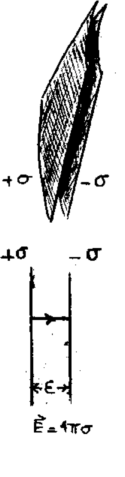
\includegraphics[width=0.2\textwidth]{images/fig_ft1_campo_dipolar3.pdf}	 
	\end{center}
	\caption{}
\end{figure}

Veamos algún detalle más sobre la capa dipolar, que está ilustrado en la Figura siguiente.
\[
	\frac{ \vb{D}\cdot(\vb{x}-\vb{x}')}{|\vb{x} - \vb{x}'|^3} dS = 
	\frac{ D \cdot(\vb{x}-\vb{x}')}{|\vb{x} - \vb{x}'|^3} d\vb{S} = 
	- \frac{ D \cos(\theta)}{|\vb{x} - \vb{x}'|^2} dS = 
	- \frac{ D \cos(\theta)}{r^2} dS  
\]

\begin{figure}[htb]
	\begin{center}
	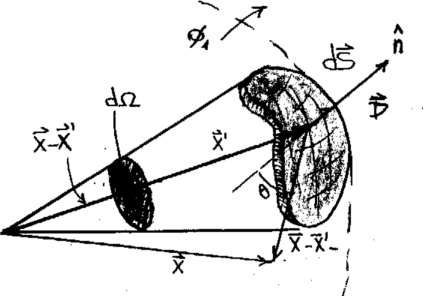
\includegraphics[width=0.6\textwidth]{images/fig_ft1_campo_dipolar1.pdf}	 
	\end{center}
	\caption{}
\end{figure}

\[
	\frac{ \vb{D}\cdot(\vb{x}-\vb{x}')}{|\vb{x} - \vb{x}'|^3} dS = - D d\Omega
\]
puesto que
\[
	\phi(\vb{x}) = -D \int_S d\Omega \qquad \qquad \frac{\cos(\theta)}{r^2}dS \equiv d\Omega
\]

Para las condiciones de contorno se da lo siguiente
\[
	E_2^{\hat{n}} - E_1^{\hat{n}} = 4\pi\sigma
\]
\[
	- \Nabla (\phi_2 - \phi_1)\cdot \hat{n} = 4\pi\sigma
\]
\[
	\dpar{\phi_1 - \phi_2}{\hat{n}} = 4\pi\sigma
\]
\[
	\phi_1 - \phi_2 = 4\pi\sigma\epsilon
\]

\begin{figure}[htb]
	\begin{center}
	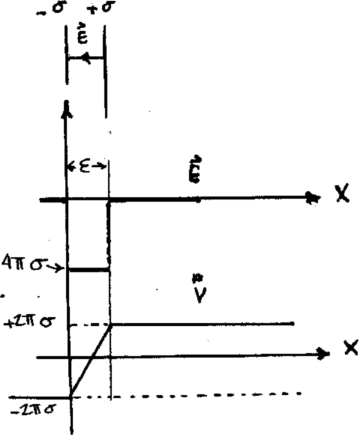
\includegraphics[width=0.4\textwidth]{images/fig_ft1_campo_dipolar2.pdf}	 
	\end{center}
	\caption{}
\end{figure}

desde donde deducimos que el potencial tiene un salto al surcar la capa dado por 
\[
	\phi_2 - \phi_1 = 4\pi D
\]

\subsection{Momento dipolar por unidad de volumen}

El potencial de un dipolo es
\[
	\phi(\vb{x}) = \frac{ \vb{p}\cdot(\vb{x}-\vb{x}') }{|\vb{x} - \vb{x}'|^3} 
\]
y el potencial de muchos de ellos sale de la integración
\[
	\phi(\vb{x}) = \int_V \frac{ \vb{P}(\vb{x}')\cdot(\vb{x}-\vb{x}') }{|\vb{x} - \vb{x}'|^3}  \: dV
\]
\begin{figure}[htb]
	\begin{center}
	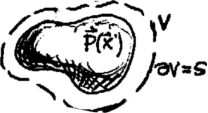
\includegraphics[width=0.3\textwidth]{images/fig_ft1_dipolarvol.pdf}	 
	\end{center}
	\caption{}
\end{figure}
donde $\vb{P}$ es la llamada polarización, el momento dipolar por unidad de volumen, siendo $V$ un volumen
que incluye a la zona de polarización (ver Figura).
\[
	\phi(\vb{x}) = \int_V \vb{P}(\vb{x}')\cdot \Nabla' \left(\frac{1}{|\vb{x} - \vb{x}'|} \right)\: dV
\]
y si usamos el teorema de la divergencia para convertir una de las integrales resulta
\[
	\phi(\vb{x}) = \int_S \frac{\vb{P}(\vb{x}')}{ |\vb{x} - \vb{x}'|} \: dS
	- \int_V  \frac{  \Nabla' \cdot \vb{P}(\vb{x}') }{|\vb{x} - \vb{x}'|} \: dV 
\]
lo que habilita a pensar en como que 
\[
	\vb{P}\cdot\hat{n} \equiv \sigma_P
\]
está presente en el borde del cuerpo polarizado, y en su interior existe
\[
	- \Nabla\cdot\vb{P} \equiv \rho_P
\]
siempre que $\divem{P}\neq 0$ es decir que la polarización no sea homogénea.

% =================================================================================================
\section{El potencial vector}
% =================================================================================================

Haremos una especie de desarrollo multipolar del potencial vector \vb{A},
\[
	\vb{A}(\vb{x}) = \frac{1}{c} \int_V \frac{\vb{J}(\vb{x}')}{|\vb{x}-\vb{x}'|} \: dV' 
\]
pero como se puede escribir
\[
	\frac{1}{|\vb{x}-\vb{x}'|} \approx \frac{1}{|\vb{x}|}  + \frac{\vb{x}\cdot\vb{x}'}{|\vb{x}|^3} 
\]
en torno a $\vb{x}'=0$ será
\notamargen{Recordar que Biot \& Savart es para densidad de corriente estacionaria,
i.e. $\divem{J}=0$}
\[
	\vb{A}(\vb{x}) = \frac{1}{c} \int_V \frac{\vb{J}(\vb{x}')}{|\vb{x}|} \: dV' 
	+ \frac{1}{c} \frac{ \vb{x} \: }{|\vb{x}|^3} \cdot \int_V \vb{x}' \vb{J}(\vb{x}') \: dV' 
\]
\[
	\vb{A}(\vb{x}) = \frac{1}{c|\vb{x}|} \int_V \vb{J}(\vb{x}') \: dV' 
	+ \frac{1}{c} \frac{ \vb{x} \: }{|\vb{x}|^3} \cdot \int_V \vb{x}' \vb{J}(\vb{x}') \: dV' 
\]
y el primer término es nulo lo cual puede verse porque sale integrando con alguna identidad (?)
y usando que $\divem{J}=0$. Correspondería al orden monopolar y el hecho de que sea nulo refleja
la no existencia de monopolos.
\[
	\vb{A}(\vb{x}) = \left[ \left(\frac{1}{2c} \int_V \vb{x}'\times \vb{J} \: dV \right) \times \vb{x} \right] 
			\frac{1}{|\vb{x}|^3}
\]
y si definimos el paréntesis como \vb{m} (momento magnético) entonces
\[
	\vb{A}(\vb{x}) = \frac{\vb{m} \times \vb{x} }{|\vb{x}|^3}
\]
en el origen, y 
\[
	\vb{A}(\vb{x}) = \frac{\vb{m} \times (\vb{x}-\vb{x}') }{|\vb{x}-\vb{x}'|^3}
\]
en $\vb{x}'$, las cuales son expresiones a primer orden y que utilizan el gauge de Coulomb, $\divem{A}=0$.

De esta manera tendremos
\[
	\mathcal{M}(\vb{x}') = \frac{1}{2c} \left[ \vb{x}' \times \vb{J}(\vb{x}')\right]
\]
que es la magnetización o densidad de momento magnético, y entonces el momento magnético pasa a ser 
\[
	\vb{m} = \int_v \mathcal{M}(\vb{x}') \:dV'.
\]

Se puede trabajar con el potencial vector así
\[
	\rotorm{A}  = \Nabla \times \left( \frac{\vb{m} \times \vb{x} }{|\vb{x}|^3} \right) =
	\left( \frac{\vb{x}}{|\vb{x}|^3}\cdot\Nabla \right)\vb{m}-(\vb{m}\cdot\Nabla)\frac{\vb{x}}{|\vb{x}|^3}, 
\]
la cual luego de mucho álgebra vectorial se puede llevar a la forma
\[
	\vb{B} = \frac{3 (\vb{m}\cdot\hat{n})\hat{n} - \vb{m}}{|\vb{x}|^3},
\]
que nos dice que bien lejos cualquier distribución de corriente localizada presenta como \vb{B} el 
campo magnético de un dipolo magnético dado por \vb{m}(\vb{x}). Esta aproximación corresponde, por 
supuesto, al primer orden del desarrollo.

\subsection{interpretacion del momento magnético}

Se puede pensar \vb{m} como una espira.
\[
	dA = \frac{ x d\ell \sin(\alpha) }{2}
\]
siendo el área orientada
\[
	\vb{A} = \frac{1}{2} \int_\Gamma \vb{x}\times d\vb{\ell} 
\]
y entonces
\[
	\vb{m} = \frac{I}{c}\vb{A}
\]
\begin{figure}[htb]
	\begin{center}
	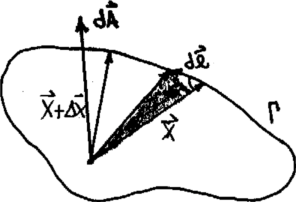
\includegraphics[width=0.5\textwidth]{images/fig_ft1_mmag.pdf}	 
	\end{center}
	\caption{}
\end{figure}

Desde volumen a espira hacemos la transformación del modo usual,
\[
	\vb{m} = \frac{1}{2c} \int_V  \vb{x} \times \vb{J}(\vb{x})  \:dV =
		\frac{1}{2c} \int_\Gamma  \vb{x} \times \:d\vb{\ell}
\]
usando que
\[
	\vb{J} \: dV = J d\vb{\ell} dS = \frac{I}{dS} d\vb{\ell} dS = I \: d\vb{\ell} 
\]

A modo de ejemplo, para una espira circular de radio $r$ es
\[
	m = \frac{i}{c} \pi r^2.
\]

\subsection{Interacción del campo magnético con una distribución de corriente}

Hacemos una expansión de Taylor del campo \vb{B} con $|\vb{x}|\ggg|\vb{x}'|$,
\[
	\vb{B} = \vb{B}_0 + (\vb{x}\cdot\Nabla)\vb{B}
\]
y entonces como la fuerza es
\[
	\vb{F} = \frac{1}{c} \int_V \vb{J}(\vb{x}') \times \vb{B}(\vb{x}') \: dV'
\]
\begin{figure}[htb]
	\begin{center}
	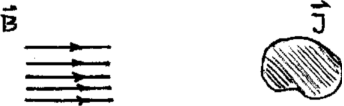
\includegraphics[width=0.5\textwidth]{images/fig_ft1_campocorr.pdf}	 
	\end{center}
	\caption{}
\end{figure}
resulta que
\[
	\vb{F} =  \frac{1}{c} \int_V \vb{J} \times \vb{B}_0 \: dV' +
		\frac{1}{c} \int_V \vb{J} \times (\vb{x}'\cdot\Nabla)\vb{B} \: dV'
\]
siendo el primer término nulo.
\[
	\vb{F} = \Nabla\times(\pv{B}{m}) = (\pe{m}{\Nabla})\vb{B} =
		(\pe{m}{\Nabla})\vb{B} = \Nabla(\pe{m}{B})
\]
Si el campo es homogéneo la fuerza es nula, pero como $\vb{F} = -\Nabla U$
\[
	F_m = \Nabla(\pe{m}{B}) \quad \Rightarrow \quad U_M = -\pe{m}{B}
\]
\[
	F_e = \Nabla(\pe{p}{E}) \quad \Rightarrow \quad U_e = -\pe{p}{E}
\]
siendo $U_{m,e}$ la energía de los dipolos en campos externos.


Mediante identidades vectoriales podemos llegar a una expresión
\[
	\vb{F} = - \Nabla \times \frac{1}{c} \int_V \vb{J}(\vb{x}'\cdot\vb{B}) dV' =
	-\Nabla \times \frac{1}{2c} (-\vb{B}) \times \int_V \vb{x} \times \vb{J} dV' =
\]
\[
	\vb{F} = \Nabla \times \vb{B} \times \frac{1}{2c}\int_V \vb{x} \times \vb{J} dV'
\]
\[
	\vb{F} = \Nabla \times (\pv{B}{m}) = \Nabla(\pe{m}{B})
\]
La fuerza de un campo $\vb{B}$ externo sobre una distribución de corrientes es el gradiente de cierta
energía
\[
	\vb{F} = \Nabla(\vb{m}\cdot\vb{B}) = (\vb{m}\cdot\Nabla)\vb{B}
\]
de donde se ve claramente que si \vb{B} es uniforme entonces la fuerza es nula.
\vb{m} es una constante que depende de la distribución de corrientes.

% =================================================================================================
\section{Pertubación por un conductor sobre un campo eléctrico uniforme}
% =================================================================================================

Se tiene un campo uniforme con $Q,R \to \infty$ pero con $2Q/R^2 = cte$, según se ve en la Figura.


El potencial $\phi$ de la esfera es constante por ser conductor.
Puedo definir 
\[
	\phi|_{esf} \equiv 0
\]
pues $\phi(\infty)\neq 0 $ porque hay densidad de carga $\rho$ en el infinito.

\begin{figure}[htb]
	\begin{center}
	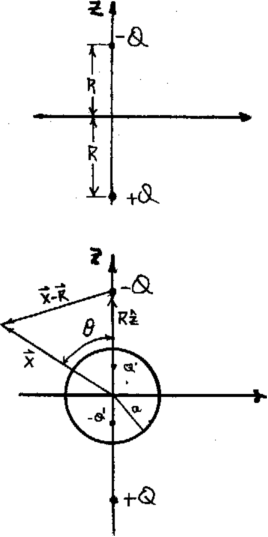
\includegraphics[width=0.4\textwidth]{images/fig_ft1_perturbacion1.pdf}	 
	\end{center}
	\caption{}
\end{figure}
Para la carga superior,
\[
	\phi_1 = \frac{-Q}{|\vb{x} - R\hat{z}|} + \frac{a/R Q}{|\vb{x} - a^2/R\hat{z}|}
\]
mientras que para la inferior
\[
	\phi_2 = \frac{Q}{|\vb{x} + R\hat{z}|} + \frac{ a/R Q}{|\vb{x} + a^2/R\hat{z}|}
\]

Recordemos que
\[
	(1+\alpha)^{(-1/2)} \approx 1 - \frac{1}{2}\alpha \qquad \alpha \ll 1
\]
y podemos trabajar el denominador
\[
	|\vb{x} - R\hat{z}| = \sqrt{ x^2 + R^2 - 2Rx\cos(\theta)}
\]
\[
	\frac{1}{|\vb{x} - R\hat{z}|} = \frac{1}{\sqrt{ x^2 + R^2 - 2Rx\cos(\theta)}} =
	\frac{1}{R(1 + x^2/R^2 - 2x/R\cos(\theta))^(1/2)}
\]
\[
	\frac{1}{|\vb{x} - R\hat{z}|} \approx \frac{1}{R}\left(1+ \frac{x}{R} \cos(\theta) \right)
\]
de manera que luego
\begin{multline*}
	\phi(r) \approx Q\left[ \frac{1}{R}\left(1+ \frac{x}{R} \cos(\theta) \right) + 
	\frac{a}{Rx}\left(1+ \frac{a^2}{Rx} \cos(\theta) \right) + \right. \\
	\left. \frac{1}{R}\left(1 - \frac{x}{R} \cos(\theta) \right) -
	\frac{a}{Rx}\left(1 - \frac{a^2}{Rx} \cos(\theta) \right) \right]
\end{multline*}
\[
	\phi(x) \approx -\frac{2Qx}{R^2} \cos(\theta) + \frac{2a^3Q}{R^2x^2}\cos(\theta)
\]
y haciendo $x\equiv r$ y tomando el límite,
\[
	\phi(r) = -E_0 r \cos(\theta) + E_0\frac{a^3}{r^2} \cos(\theta)
\]
y la carga total sobre la esfera es nula puesto que estuvo aislada todo el tiempo.
Respecto de la Figura, si hacemos un Gauss en la zona indicada se obtiene $Q_n=0$,
entonces $\phi(r=a)=0$.

\begin{figure}[htb]
	\begin{center}
	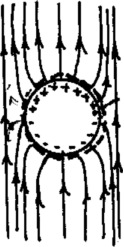
\includegraphics[width=0.2\textwidth]{images/fig_ft1_perturbacion3.pdf}	 
	\end{center}
	\caption{}
\end{figure}

El segundo término es como un dipolo puntual,
\[
	E_0\frac{a^3}{r^2} \cos(\theta) = E_0\frac{a^3 \hat{z}\cdot\vb{r}}{r^3} 
\]
donde
\[
	\vb{p} \equiv E_0 a^3 \hat{z}
\]











































































































% \bibliographystyle{CBFT-apa-good}	% (uses file "apa-good.bst")
% \bibliography{CBFT.Referencias} % La base de datos bibliográfica

\end{document}
